% Options for packages loaded elsewhere
\PassOptionsToPackage{unicode}{hyperref}
\PassOptionsToPackage{hyphens}{url}
%
\documentclass[
  ignorenonframetext,
  aspectratio=1610,
]{beamer}
\usepackage{pgfpages}
\setbeamertemplate{caption}[numbered]
\setbeamertemplate{caption label separator}{: }
\setbeamercolor{caption name}{fg=normal text.fg}
\beamertemplatenavigationsymbolsempty
% Prevent slide breaks in the middle of a paragraph
\widowpenalties 1 10000
\raggedbottom
\setbeamertemplate{part page}{
  \centering
  \begin{beamercolorbox}[sep=16pt,center]{part title}
    \usebeamerfont{part title}\insertpart\par
  \end{beamercolorbox}
}
\setbeamertemplate{section page}{
  \centering
  \begin{beamercolorbox}[sep=12pt,center]{part title}
    \usebeamerfont{section title}\insertsection\par
  \end{beamercolorbox}
}
\setbeamertemplate{subsection page}{
  \centering
  \begin{beamercolorbox}[sep=8pt,center]{part title}
    \usebeamerfont{subsection title}\insertsubsection\par
  \end{beamercolorbox}
}
\AtBeginPart{
  \frame{\partpage}
}
\AtBeginSection{
  \ifbibliography
  \else
    \frame{\sectionpage}
  \fi
}
\AtBeginSubsection{
  \frame{\subsectionpage}
}
\usepackage{amsmath,amssymb}
\usepackage{iftex}
\ifPDFTeX
  \usepackage[T1]{fontenc}
  \usepackage[utf8]{inputenc}
  \usepackage{textcomp} % provide euro and other symbols
\else % if luatex or xetex
  \usepackage{unicode-math} % this also loads fontspec
  \defaultfontfeatures{Scale=MatchLowercase}
  \defaultfontfeatures[\rmfamily]{Ligatures=TeX,Scale=1}
\fi
\usepackage{lmodern}
\ifPDFTeX\else
  % xetex/luatex font selection
\fi
% Use upquote if available, for straight quotes in verbatim environments
\IfFileExists{upquote.sty}{\usepackage{upquote}}{}
\IfFileExists{microtype.sty}{% use microtype if available
  \usepackage[]{microtype}
  \UseMicrotypeSet[protrusion]{basicmath} % disable protrusion for tt fonts
}{}
\makeatletter
\@ifundefined{KOMAClassName}{% if non-KOMA class
  \IfFileExists{parskip.sty}{%
    \usepackage{parskip}
  }{% else
    \setlength{\parindent}{0pt}
    \setlength{\parskip}{6pt plus 2pt minus 1pt}}
}{% if KOMA class
  \KOMAoptions{parskip=half}}
\makeatother
\usepackage{xcolor}
\newif\ifbibliography
\usepackage{graphicx}
\makeatletter
\def\maxwidth{\ifdim\Gin@nat@width>\linewidth\linewidth\else\Gin@nat@width\fi}
\def\maxheight{\ifdim\Gin@nat@height>\textheight\textheight\else\Gin@nat@height\fi}
\makeatother
% Scale images if necessary, so that they will not overflow the page
% margins by default, and it is still possible to overwrite the defaults
% using explicit options in \includegraphics[width, height, ...]{}
\setkeys{Gin}{width=\maxwidth,height=\maxheight,keepaspectratio}
% Set default figure placement to htbp
\makeatletter
\def\fps@figure{htbp}
\makeatother
\setlength{\emergencystretch}{3em} % prevent overfull lines
\providecommand{\tightlist}{%
  \setlength{\itemsep}{0pt}\setlength{\parskip}{0pt}}
\setcounter{secnumdepth}{-\maxdimen} % remove section numbering
\ifLuaTeX
\usepackage[bidi=basic]{babel}
\else
\usepackage[bidi=default]{babel}
\fi
\babelprovide[main,import]{english}
% get rid of language-specific shorthands (see #6817):
\let\LanguageShortHands\languageshorthands
\def\languageshorthands#1{}
\usepackage{pgfpages}
\usepackage{microtype}
\usepackage{tikz}
  \usetikzlibrary{positioning}
  \usetikzlibrary{arrows}
  \usetikzlibrary{graphs}

\definecolor{CTred}{RGB}{229,32,32}
\definecolor{CTgrey}{RGB}{153,153,153}

\usepackage{array}
\usepackage{dcolumn}
\newcolumntype{d}{D{.}{.}{-1}}
\usepackage{booktabs}
\usepackage{threeparttable}

% Redefine the section command
\let\oldsection\section
\renewcommand{\section}{
  \addtocounter{framenumber}{-1} % Decrement frame counter
  \oldsection
}
% colors: white text on 90% black background
\setbeamercolor{normal text}{fg=black,bg=white}

% light blue as a highlight color
\setbeamercolor*{structure}{fg=CTred}
\setbeamercolor{section title}{fg=CTred}
\setbeamercolor{alerted text}{use=structure,fg=CTred}
\setbeamercolor*{palette primary}{use=structure,fg=structure.fg}
\setbeamercolor*{palette secondary}{use=structure,fg=structure.fg!95!black}
\setbeamercolor*{palette tertiary}{use=structure,fg=structure.fg!90!black}
\setbeamercolor*{palette quaternary}{use=structure,fg=structure.fg!95!black,bg=black!80}

\setbeamercolor*{framesubtitle}{fg=white}


% use system fonts: here, Gill Sans
\usefonttheme{professionalfonts}
\setbeamerfont{quote}{shape=\upshape}

% eliminate silly beamer navigation line at bottom of slides
\setbeamertemplate{navigation symbols}{}
\setbeamertemplate{footline}[frame number]

% ensure text jusfication
\usepackage{ragged2e}
\justifying

% pandoc makes 2nd-lever headers into blocks, and this ensures justification
% in blocks too
\addtobeamertemplate{block begin}{}{\justifying}




\urlstyle{same}
\usepackage[overlay,absolute]{textpos}

\setbeamertemplate{items}[square]

\TPGrid[10 mm,8 mm]{9}{8}
% beamer's left and right margin is 10 mm. The top/bottom margin is ??
% or without a header ??
% the slide dimensions are 128 mm x 96 mm
% so the resulting \TPHorizModule = 12 mm and \TPVertModule = 10 mm

% uncomment if you want biblatex for citations on slides

% \usepackage{csquotes}
% \usepackage[notes,short,noibid,backend=biber]{biblatex-chicago}
% \bibliography{course.bib} 

\providecommand{\exhibit}[2]{\includegraphics[keepaspectratio, height=0.9\textheight, width=\textwidth]{assets/img/#1}\\ {\tiny #2}}

\providecommand{\smallcite}[1]{({\footnotesize #1})}
\ifLuaTeX
  \usepackage{selnolig}  % disable illegal ligatures
\fi
\IfFileExists{bookmark.sty}{\usepackage{bookmark}}{\usepackage{hyperref}}
\IfFileExists{xurl.sty}{\usepackage{xurl}}{} % add URL line breaks if available
\urlstyle{same}
\hypersetup{
  pdftitle={The Macroeconomics of Managers: Supply, Selection and Competition},
  pdfauthor={Miklós Koren (CEU, KRTK, CEPR and CESifo); Krisztina Orbán (Monash)},
  pdflang={en},
  hidelinks,
  pdfcreator={LaTeX via pandoc}}

\title{The Macroeconomics of Managers: Supply, Selection and
Competition}
\author{Miklós Koren (CEU, KRTK, CEPR and CESifo) \and Krisztina Orbán
(Monash)}
\date{December 14, 2023\footnote<.->{Supported by Forefront Research
  Excellence Grant (144193) and ERC Advanced Grant (101097789)}}

\begin{document}
\frame{\titlepage}

\section{Introduction}\label{introduction}

\begin{frame}{Hungary, 1980 (Fortepan / Szalay Zoltán)}
\protect\hypertarget{hungary-1980-fortepan-szalay-zoltuxe1n}{}
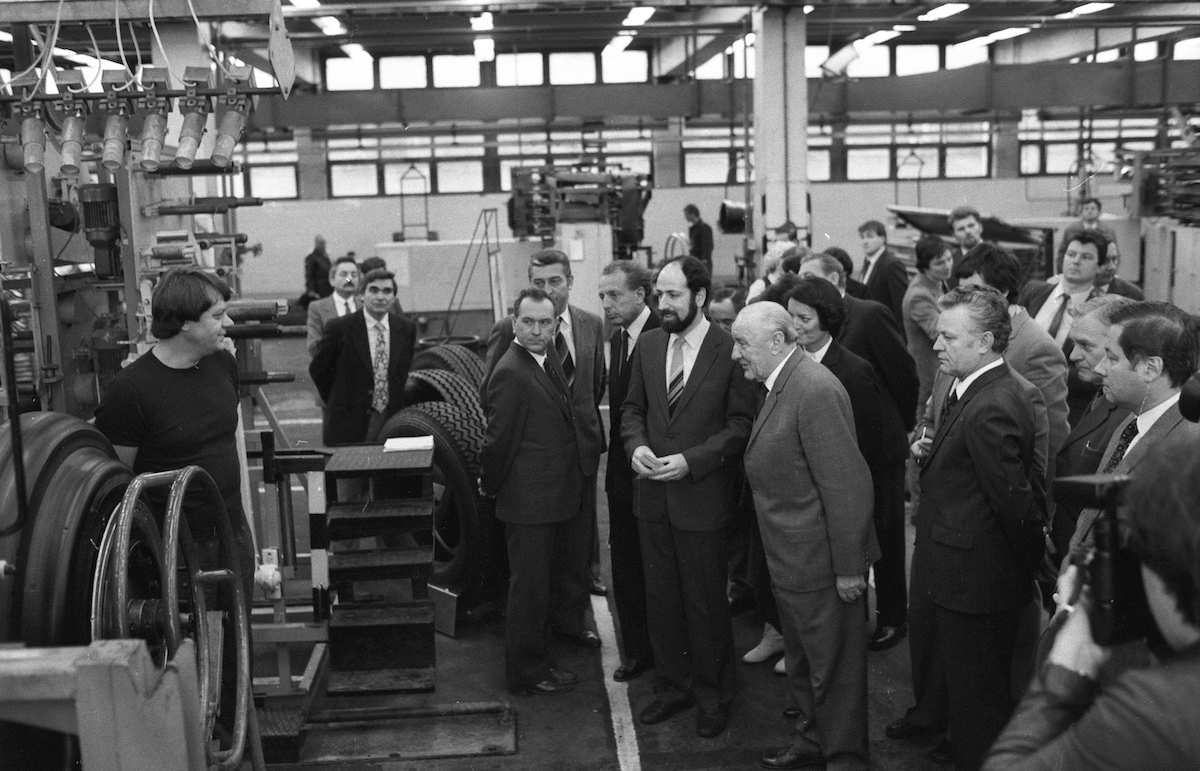
\includegraphics{fig/fortepan_198036.jpg}
\end{frame}

\begin{frame}{Hungary, 1990 (MTI)}
\protect\hypertarget{hungary-1990-mti}{}
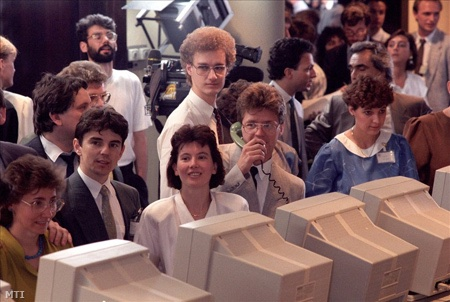
\includegraphics{fig/tozsde.jpg}
\end{frame}

\begin{frame}{Number of Executive Positions Increased}
\protect\hypertarget{number-of-executive-positions-increased}{}
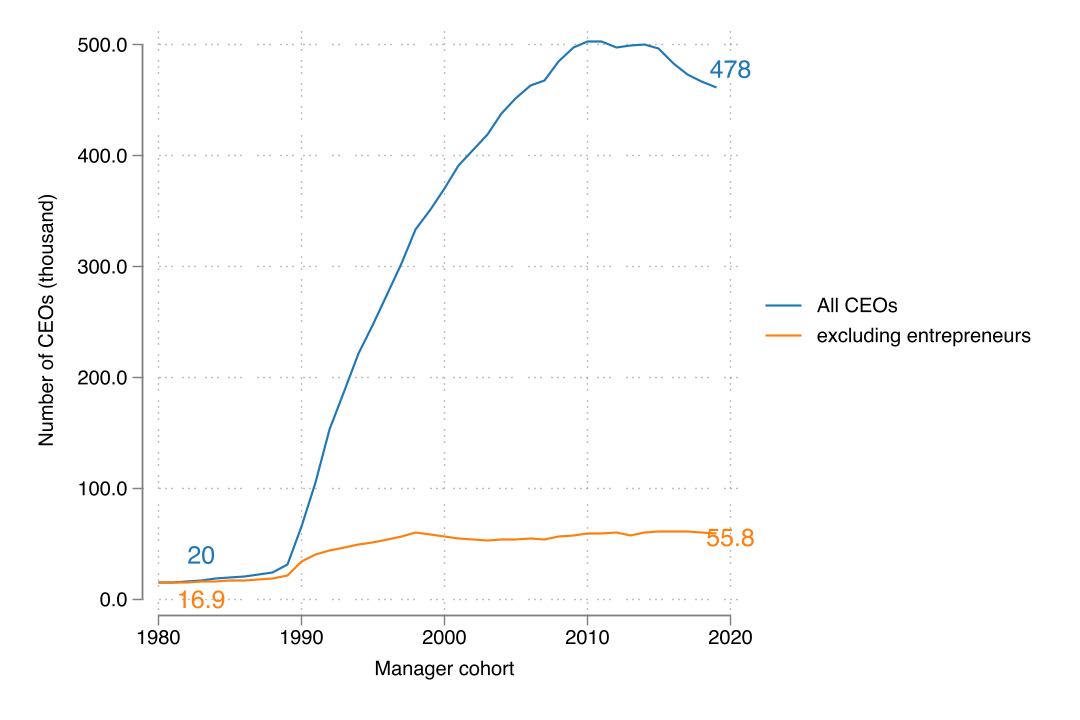
\includegraphics{fig/ceo-stock.png}
\end{frame}

\begin{frame}{Business Degrees Became More Prominent}
\protect\hypertarget{business-degrees-became-more-prominent}{}
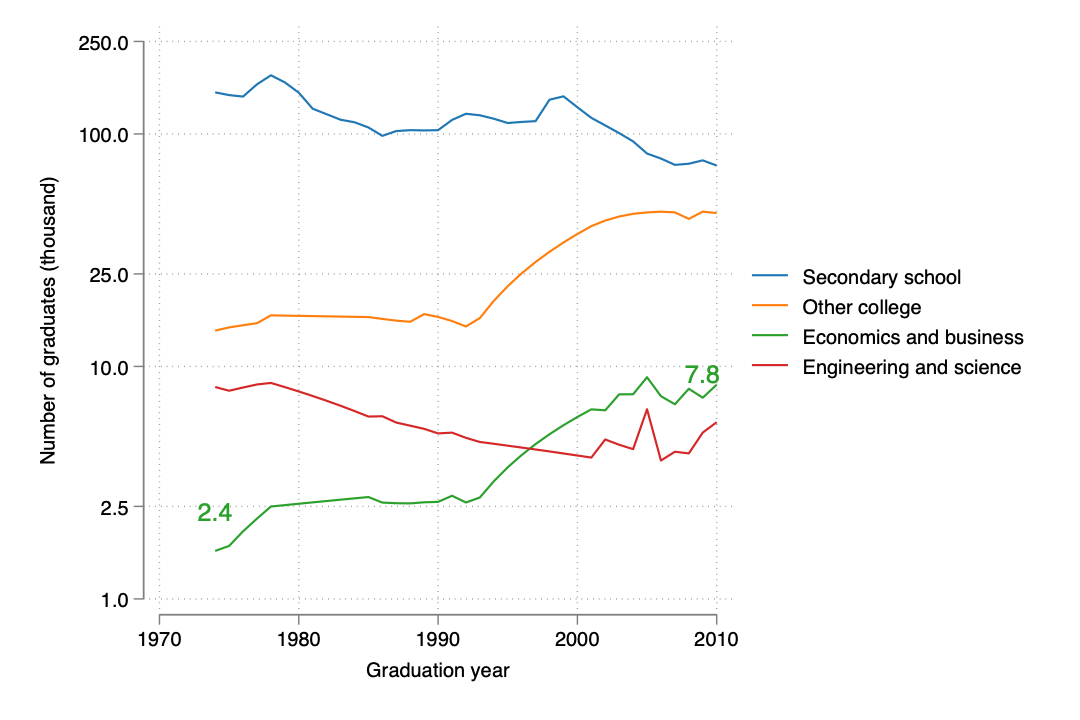
\includegraphics{fig/school-graduates.png}
\end{frame}

\begin{frame}{What Can We Learn From Hungary?}
\protect\hypertarget{what-can-we-learn-from-hungary}{}
Use Hungarian post-socialist transition as a natural experiment to study
the supply side of the market for managers.
\end{frame}

\begin{frame}{Why Micro \(\neq\) Macro}
\protect\hypertarget{why-micro-neq-macro}{}
\begin{block}{What we know}
\protect\hypertarget{what-we-know}{}
\begin{enumerate}
\tightlist
\item
  Management matters
\item
  Training works
\item
  Managers matter
\end{enumerate}

\pause
\end{block}

\begin{block}{What we don't know}
\protect\hypertarget{what-we-dont-know}{}
\begin{enumerate}
\tightlist
\item
  What policy interventions can improve management for an entire
  country?
\item
  How to quantify the macro effects of these policies?
\end{enumerate}

\pause
\end{block}

\begin{block}{What we need}
\protect\hypertarget{what-we-need}{}
\begin{enumerate}
\tightlist
\item
  Endogenous supply: how to incentivize people to become managers?
\item
  Selection: who will become managers?
\item
  Competition: what are the GE feedbacks of interventions?
\end{enumerate}
\end{block}
\end{frame}

\section{Setup and Data}\label{setup-and-data}

\begin{frame}{Data}
\protect\hypertarget{data}{}
\begin{block}{Manager Data 1985-2019}
\protect\hypertarget{manager-data-1985-2019}{}
Universe of corporations (1m) and their CEOs (1.3m). Firm size
(employment) as proxy for manager quality.
\end{block}

\begin{block}{Biographies}
\protect\hypertarget{biographies}{}
Full biographies (school, work experience, etc.) for 63k people in 2013.
30k matched to CEO panel.
\end{block}

\begin{block}{College graduates}
\protect\hypertarget{college-graduates}{}
Number of gradues by degree and year.
\end{block}
\end{frame}

\begin{frame}{Quantity Up, Quality Down}
\protect\hypertarget{quantity-up-quality-down}{}
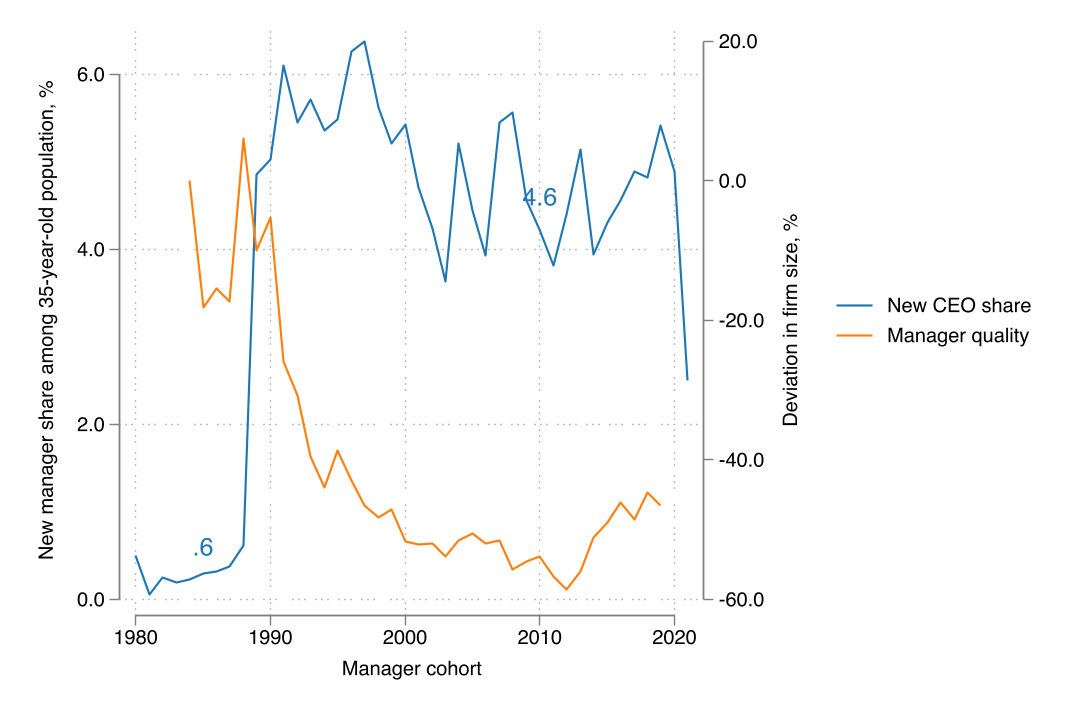
\includegraphics{fig/ceo-flow-with-FE.png}
\end{frame}

\section{An Equilibrium Model of
Managers}\label{an-equilibrium-model-of-managers}

\begin{frame}{An Equilibrium Model of Managers}
\protect\hypertarget{an-equilibrium-model-of-managers-1}{}
\begin{enumerate}
\tightlist
\item
  Managers have innate skill and can be trained (at university).
\item
  Schooling responds to incentives.
\item
  Self-selection into management based on skill (frictions + dynamics).
\item
  Wages determined in equilibrium.
\end{enumerate}
\end{frame}

\begin{frame}{Production Function}
\protect\hypertarget{production-function}{}
A manager with skill \(z\) can hire \(l\) workers to produce output
\[q = z^\nu l^{1-\nu}.\]

\pause

Aggregate GDP: \[Y = Z^\nu {L^{p}}^{1-\nu}\] with sum of manager skills
\[Z = N\cdot \tilde z = N\cdot\int\! z dG(z)\]

\pause

Policy goal: Increase \(Z\) via either \(N\) (more managers) or
\(\bar z\) (better training).
\end{frame}

\begin{frame}{Corporate Governance Friction}
\protect\hypertarget{corporate-governance-friction}{}
Operating surplus, \[\Pi(z) = q(z) - w l(z) = z \pi(w) \] linear in
\(z\). Worker wage (\(w\)) is endogenous. \pause

\textbf{Owners cannot commit to sharing more than a fraction of
surplus}.

Manager wage is \[
\omega(z) \le \phi \Pi(z) = \phi z \pi(w) 
\] with \(\phi < 1\).

\textbf{Underprovision of manager skills.}
\end{frame}

\begin{frame}{Education and Career Choice}
\protect\hypertarget{education-and-career-choice}{}
\begin{block}{Career Choice}
\protect\hypertarget{career-choice}{}
Manager if \(\omega(z) > w\), \[ z > z_{\min}(Z).\]
\end{block}

\begin{block}{Education}
\protect\hypertarget{education}{}
Different degrees lead to different \(z\) distributions (Pareto).
Discrete choice over degrees given tuition, expected income, and
non-pecuniary preferences.
\end{block}
\end{frame}

\begin{frame}{What Can Policy Do?}
\protect\hypertarget{what-can-policy-do}{}
\begin{enumerate}
\tightlist
\item
  Reduce corporate governance frictions.
\item
  Subsidize business schools.
\item
  Reform business school curriculum.
\end{enumerate}
\end{frame}

\begin{frame}{A Taxonomy of Equilibrium Feedback Effects}
\protect\hypertarget{a-taxonomy-of-equilibrium-feedback-effects}{}
\begin{block}{Supply}
\protect\hypertarget{supply}{}
Higher share going to business schools, more managers
\end{block}

\begin{block}{Selection}
\protect\hypertarget{selection}{}
Different innate ability of managers, \emph{conditional} on school
choice
\end{block}

\begin{block}{Competition}
\protect\hypertarget{competition}{}
Worker and manager wages respond to entry of new managers
\end{block}
\end{frame}

\begin{frame}{Steady State Results}
\protect\hypertarget{steady-state-results}{}
\begin{block}{Manager share}
\protect\hypertarget{manager-share}{}
\[
\frac{N_*}{L} = \frac 1{1+  
\frac {1-\nu}{\phi\nu}
\frac {\theta}{\theta - 1}}
\] with \(\theta>1\) the shape of the Pareto skill distribution.

\pause
\end{block}

\begin{block}{Value added per worker}
\protect\hypertarget{value-added-per-worker}{}
\[
\frac{Y_*}{L} = 
\left(\frac{\nu}{1-\nu} \right)^\nu
\phi^\nu
(\Lambda_* z_0)^\nu
\left(\frac {N_*}{L}
\right)^{-\nu/\theta}
\left(1-\frac {N_*}{L}
\right)
\] with
\(\Lambda_* = \left[\sum_i x_i \lambda_i^\theta \right]^{1/\theta}\) the
average skill multiplier across degrees.
\end{block}
\end{frame}

\section{Taking the Model to the
Data}\label{taking-the-model-to-the-data}

\begin{frame}{Goal}
\protect\hypertarget{goal}{}
Calibrate model to match two steady states:

\begin{enumerate}
\tightlist
\item
  communism (-1989)
\item
  capitalism (2005-2010)
\end{enumerate}

with only one change, \(\phi_0 \to \phi_1\).
\end{frame}

\begin{frame}{Calibration}
\protect\hypertarget{calibration}{}
\begin{table}[ht!]
\centering
\caption{Calibrated parameter values}   
\begin{tabular}{clr}
  \hline
Parameter & Explanation & Value \\
    \hline
$\nu$ & Steady-state ratio of managers to workers & 0.174 \\
$\phi_0$ & Surplus sharing under communism & 0.130 \\
$\phi_1$ & Surplus sharing under capitalism & 1.000 \\
$\theta$ & Skill distribution, shape & 6.87 \\
$\lambda_1$ & Skill multiplier in business school & 1.80 \\
$\lambda_2$ & Skill multiplier in engineering & 1.71 \\
$\lambda_3$ & Skill multiplier in other college & 1.35 \\
$\gamma$ & Importance of non-pecuniary education benefits & 0.06 \\
    \hline
\end{tabular}
\end{table}
\end{frame}

\begin{frame}{Policy Counterfactuals}
\protect\hypertarget{policy-counterfactuals}{}
\begin{enumerate}
\tightlist
\item
  \textbf{Transition}: Increase \(\phi\) to 1 suddenly.
\item
  \textbf{Manager subsidy}: Increase \(\phi\) to increase GDP by 5
  percent.
\item
  \textbf{School benefit}: Increase \(\alpha_i\) to increase GDP by 5
  percent.
\item
  \textbf{Curriculum reform}: Increase \(\lambda_i\) to increase GDP by
  5 percent.
\end{enumerate}
\end{frame}

\begin{frame}{Policy Counterfactuals}
\protect\hypertarget{policy-counterfactuals-1}{}
\begin{tabular}{lcccc}
\toprule
{} & Transition & Manager subsidy & School benefit & Curriculum \\
\midrule
Percentage change        &                &        41.5 &       28.0 &           41.8 \\
Manager entry            &           49.1 &         7.0 &         0.0 &            0.0 \\
Average education        &            1.6 &         0.2 &         5.0 &            5.0 \\
Selection                &           -5.2 &        -1.0 &         0.0 &            0.0 \\
Competition              &          -15.0 &        -1.1 &         0.0 &            0.0 \\
\midrule
Total GDP change         &           22.1 &         5.0 &         5.0 &            5.0 \\
\midrule
Share in business school &          10.6 &       4.0 &       72.0 &          6.0 \\
\bottomrule
\end{tabular}
\end{frame}

\section{Conclusion}\label{conclusion}

\begin{frame}{Results}
\protect\hypertarget{results}{}
\begin{itemize}
\tightlist
\item
  Transition results in ``gold rush'' of managers and business schools.
\item
  Every policy faces strong pushback from selection and competition.
\item
  Curriculum reform has most direct effect.
\end{itemize}
\end{frame}

\begin{frame}{Contributions}
\protect\hypertarget{contributions}{}
\begin{itemize}
\tightlist
\item
  Tractable, quantifiable model of manager demand and supply.
\item
  Novel data for Hungary, 1985-2019.
\item
  Use transition as macro shock to identify macro model.
\end{itemize}
\end{frame}

\section{Appendix}\label{appendix}

\begin{frame}{Literature}
\protect\hypertarget{literature}{}
\begin{itemize}
\tightlist
\item
  Large-scale management interventions: Italy (Giorcelli 2019), US
  (Bianchi and Giorcelli 2022, Giorcelli 2023)
\item
  Large-scale education interventions: Italy (Bianchi and Giorcelli
  2020), Colombia (Ferreyra et al 2023), Vietnam (Vu 2023)
\item
  Selection by skill: Denmark (Akcigit, Pearce and Prato 2020)
\item
  Calibrated models with education and selection: Guner et al 2008,
  Bhattacharya et al.~2013, Gomes and Kuehn 2017 and Esfahani 2019.
\end{itemize}
\end{frame}

\section{Education and Career
Choice}\label{education-and-career-choice-1}

\begin{frame}{Education and Career Choice}
\protect\hypertarget{education-and-career-choice-2}{}
\begin{enumerate}
\tightlist
\item
  Choose school \(i\)
\item
  Draw innate manager skill \(z\)
\item
  Get trained in school: \(z\to\lambda_i z\)
\item
  Choose whether manager or worker
\end{enumerate}

We solve the model backwards.
\end{frame}

\begin{frame}{Distribution of Manager Skills}
\protect\hypertarget{distribution-of-manager-skills}{}
We assume that \(z\) is distributed Pareto, depending on schooling
\[1-F_i(x) = \Pr(z > x|\text{school}=i) = \left(\frac x{\lambda_i z_0}\right)^{-\theta}\]
for \(\theta>1\) (so that the distribution has a finite mean).
\end{frame}

\begin{frame}{Career Choice After Graduation}
\protect\hypertarget{career-choice-after-graduation}{}
Potential managers choose to enter if net value exceeds the opportunity
cost, \[\phi v(t)z > J(t)\] Selection on manager skill,
\[z > z_{\min}(t) := \frac {J(t)} {\phi v(t)}.\]

Entry cutoff \(z_{\min}\) independent of school \(i\).
\end{frame}

\begin{frame}{Expected Career When Entering School}
\protect\hypertarget{expected-career-when-entering-school}{}
Schools affect

\begin{enumerate}
\tightlist
\item
  the probability of becoming a manager
\item
  expected skills and wages
\end{enumerate}
\end{frame}

\begin{frame}{Probability of becoming a manager}
\protect\hypertarget{probability-of-becoming-a-manager}{}
\[
\pi_i(t) = 
    z_{\min}(t)^{-\theta}
        (\lambda_i z_0)^{\theta}
\]
\end{frame}

\begin{frame}{Average manager skills}
\protect\hypertarget{average-manager-skills}{}
\[\tilde z(t) = \frac {\theta}{\theta-1} z_{\min}(t) \]
\end{frame}

\begin{frame}{Manager Value}
\protect\hypertarget{manager-value}{}
Bellman equation for manager value:
\[\rho V(t,z) = \omega[z,Z(t)] - \delta V(t,z) + V_t(t,z)\] Guess
solution: \[V(t,z) = v(t)z\] If this is the case, the Bellman can be
rewritten as
\[\rho v(t) = \nu p \left[\frac {L^{p}(t)}{Z(t)}\right]^{1-\nu} - \delta v(t) + v'(t)\]
\end{frame}

\begin{frame}{Expected labor income from a degree}
\protect\hypertarget{expected-labor-income-from-a-degree}{}
\begin{multline*}
E_i(t) = 
\pi_i(t)\phi v(t) \tilde z(t) + [1-\pi_i(t)] J(t) = \\
J(t) \left[
1 + (\lambda_i z_0)^\theta \phi^{\theta} v(t)^\theta J(t)^{-\theta}/(\theta-1)
\right]
\end{multline*}
\end{frame}

\begin{frame}{Probability of choosing school \(i\)}
\protect\hypertarget{probability-of-choosing-school-i}{}
\[
x_i = \frac {e^{\alpha_i} \left[
1 + (\lambda_i z_0)^\theta \phi^{\theta} v(t)^\theta J(t)^{-\theta}/(\theta-1)
\right]^{1/\gamma}   } 
{\sum_j e^{\alpha_j}\left[
1 + (\lambda_j z_0)^\theta \phi^{\theta} v(t)^\theta J(t)^{-\theta}/(\theta-1)
\right]^{1/\gamma}   }.
\]

\(1/\gamma\): elasticity of school choice

\(\alpha_i\): attractiveness of school \(i\)
\end{frame}

\begin{frame}{Aggregate skill level}
\protect\hypertarget{aggregate-skill-level}{}
\[
\Lambda(t) = \left[\sum_i x_i \lambda_i^\theta \right]^{1/\theta}
\]
\end{frame}

\section{Demographics}\label{demographics}

\begin{frame}{Manager and Worker Demographics}
\protect\hypertarget{manager-and-worker-demographics}{}
Workers and managers die at a constant rate \(\delta\).

The stock of population: \[
L := \int_{-\infty}^t e^{\delta{(s-t)}}l ds = l/\delta.
\] The mass of active managers: \[
N(t) := \int_{-\infty}^t e^{\delta{(s-t)}}n(s) ds.
\] The stock of workers: \[L^{p} (t) := L-N(t)\]
\end{frame}

\begin{frame}{Competition Between Firms}
\protect\hypertarget{competition-between-firms}{}
Potential new managers have a time invariant skill distribution
\(F(z)\).

Only the best become managers: a time varying truncation of \(F\).

The distribution of skill among the stock of managers, denoted by
\(G(t, z)\), is a mixture of these truncated distributions.
\end{frame}

\section{Dynamics}\label{dynamics}

\begin{frame}{Dynamics}
\protect\hypertarget{dynamics-1}{}
Bellman equation of manager wages
\[v'(t) = (\rho+\delta) v(t) - \nu \left[\frac {L^{p}(t)}{Z(t)}\right]^{1-\nu}\]
The set of managers will be a slowly moving state variable.
\[N'(t) = n(t) - \delta N(t)\] The change in the overall skill of
managers is \[Z'(t) = n(t)\tilde z(t) - \delta Z(t)\] The change in the
discounted PV of worker wages is \[J'(t)=(\rho+\delta)J(t)-w(t)\]
\end{frame}

\begin{frame}{Dynamic Equilibrium}
\protect\hypertarget{dynamic-equilibrium}{}
Ordinary differential equations in \(Z\) and \(N\) (state) and \(v\) and
\(J\) (co-state):

\begin{align*}
v'(t) &= (\rho+\delta) v(t) - \nu \left[\frac {L - N(t)}{Z(t)}\right]^{1-\nu} \\
Z'(t) &= \frac{\theta}{\theta-1} \delta L [\Lambda(t)z_0]^\theta \phi^{\theta-1} [v(t)/J(t)]^{\theta-1} - \delta Z(t) \\
N'(t) &= \delta L [\Lambda(t)z_0]^\theta \phi^{\theta} [v(t)/J(t)]^\theta - \delta N(t) \\
J'(t) &= (\rho+\delta) J(t) - (1-\nu) \left[\frac {L - N(t)}{Z(t)}\right]^{-\nu}
\end{align*}
\end{frame}

\begin{frame}{Transitional Dynamics}
\protect\hypertarget{transitional-dynamics}{}
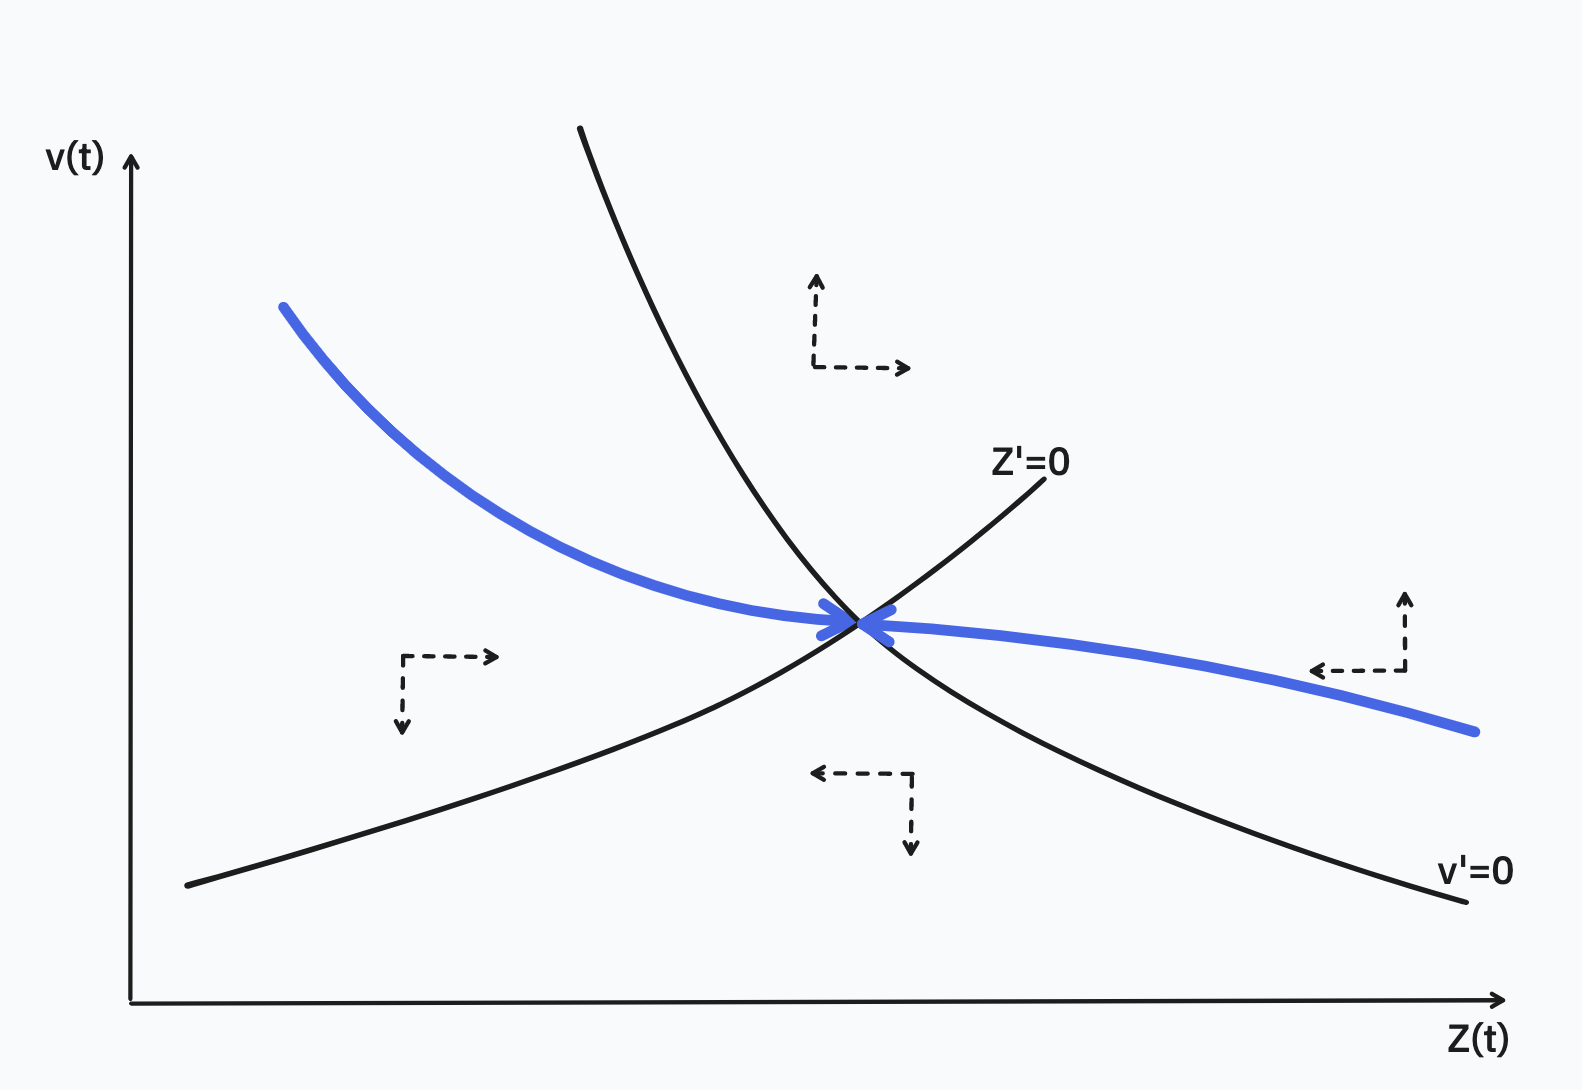
\includegraphics{fig/phase1.png}
\end{frame}

\begin{frame}{Transition: Manager entry increases suddenly}
\protect\hypertarget{transition-manager-entry-increases-suddenly}{}
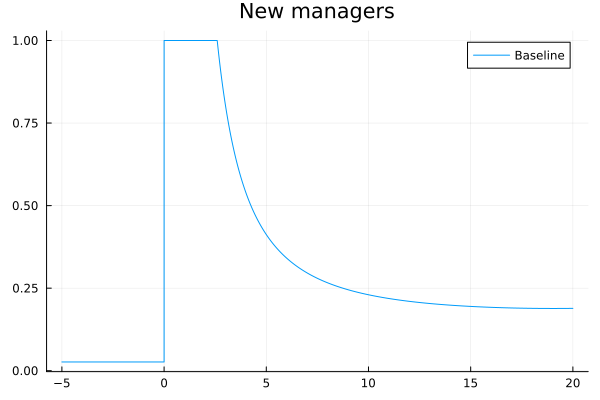
\includegraphics[width=13cm,height=8cm]{fig/model-entry-liberalization.png}
\end{frame}

\begin{frame}{Transition: Entrant skill drops sharply}
\protect\hypertarget{transition-entrant-skill-drops-sharply}{}
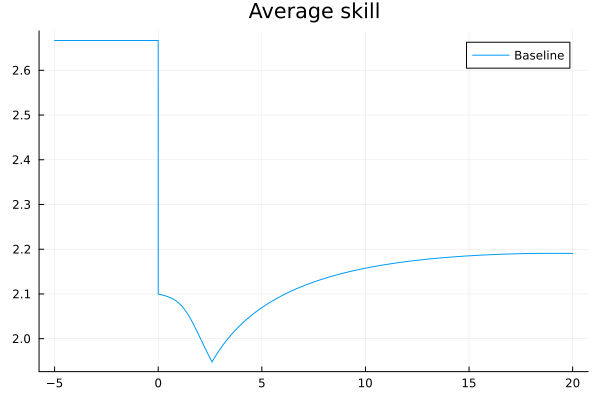
\includegraphics[width=13cm,height=8cm]{fig/model-skill-liberalization.png}
\end{frame}

\begin{frame}{Transition: Business schools become more popular}
\protect\hypertarget{transition-business-schools-become-more-popular}{}
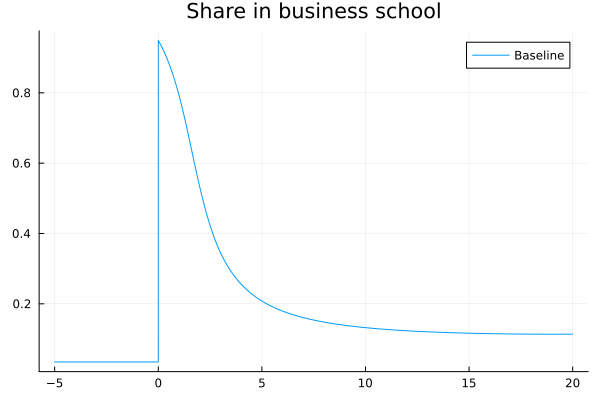
\includegraphics[width=13cm,height=8cm]{fig/model-econ-liberalization.png}
\end{frame}

\begin{frame}{Transition: GDP converges to a higher steady state}
\protect\hypertarget{transition-gdp-converges-to-a-higher-steady-state}{}
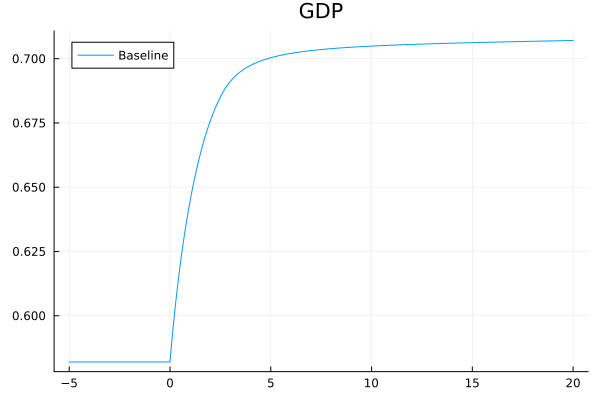
\includegraphics[width=13cm,height=8cm]{fig/model-gdp-liberalization.png}
\end{frame}

\section{Measuring Manager Quality}\label{measuring-manager-quality}

\begin{frame}{Measuring Manager Quality}
\protect\hypertarget{measuring-manager-quality-1}{}
Log employment of firm \(i\) in year \(t\) in industry \(s\), with a
mananager having entered in cohort \(c\) is \[
\ln L_{icst} = \beta_1\text{manager\_age}_{ict} + \beta_2\text{firm\_age}_{ict}  + \mu_{c} + \xi_{st} + \epsilon_{ict}.
\]

Quality: \(\mu_c\)
\end{frame}

\begin{frame}{Degree of Selection}
\protect\hypertarget{degree-of-selection}{}
\[
\ln \pi_{ic} = \theta\ln\lambda_i  - \theta \mu_c + \varepsilon_{ic}.
\]

Selectivity: \(\theta\)
\end{frame}

\begin{frame}{Manager Selection by Degree}
\protect\hypertarget{manager-selection-by-degree}{}
\begin{center}
\begin{tabular}{lc} \hline
 & (1) \\
VARIABLES & ln\_pi \\ \hline
\vspace{4pt} & \begin{footnotesize}\end{footnotesize} \\
(firstnm) firm\_size & -6.872*** \\
\vspace{4pt} & \begin{footnotesize}(1.982)\end{footnotesize} \\
(firstnm) degree = 1, economics & 4.032*** \\
\vspace{4pt} & \begin{footnotesize}(0.368)\end{footnotesize} \\
(firstnm) degree = 2, engineering & 3.676*** \\
\vspace{4pt} & \begin{footnotesize}(0.492)\end{footnotesize} \\
(firstnm) degree = 3, other & 2.041*** \\
\vspace{4pt} & \begin{footnotesize}(0.455)\end{footnotesize} \\
Constant & -14.92*** \\
 & \begin{footnotesize}(2.106)\end{footnotesize} \\
\vspace{4pt} & \begin{footnotesize}\end{footnotesize} \\
Observations & 87 \\
 $R^2$ & 0.553 \\ \hline
\multicolumn{2}{c}{\begin{footnotesize} Robust standard errors in parentheses\end{footnotesize}} \\
\multicolumn{2}{c}{\begin{footnotesize} *** p$<$0.01, ** p$<$0.05, * p$<$0.1\end{footnotesize}} \\
\end{tabular}
\end{center}

\end{frame}

\end{document}
